\chapter{Referencial Teórico}
\label{cap:referencial_teorico}

Este capítulo reúne os conceitos que sustentam a pesquisa, organizados em cinco seções. A Seção~\ref{sec:ref_eng_software_experimental} trata da Engenharia de Software Experimental e do estudo de caso, método central desta monografia. A Seção~\ref{sec:ref_qualidade_seguranca} situa a segurança entre os atributos de qualidade de software. A Seção~\ref{sec:ref_cloud_native} apresenta as arquiteturas nativas em nuvem e a orquestração de contêineres. A Seção~\ref{sec:ref_monitoramento_logs} aborda o monitoramento em tempo de execução e a gestão de registros de auditoria. Por fim, a Seção~\ref{sec:ref_conformidade_normativa} descreve o arcabouço normativo federal que fornece os critérios de avaliação do estudo.

\section{Engenharia de Software Experimental}
\label{sec:ref_eng_software_experimental}

A Engenharia de Software é uma área multidisciplinar, que reúne questões técnicas, como sistemas operacionais e bancos de dados, e questões sociais e psicológicas, e cujo desenvolvimento depende fortemente da atividade humana \cite{wohlin2024}. Por essa razão, não se espera encontrar leis formais comparáveis às da Física, exceto em aspectos estritamente técnicos, e as decisões sobre como desenvolver software precisam ser sustentadas por métodos científicos \cite{wohlin2024}. A Engenharia de Software Experimental fornece esse conjunto de métodos.

Entre as abordagens gerais de pesquisa na área, sintetizadas por \citeonline{wohlin2024} como científica, de engenharia, empírica e analítica, interessa a este trabalho a abordagem empírica, na qual uma proposta ou um modelo é avaliado por meio de estudos empíricos. A Tabela~\ref{tab:ref_abordagens_empiricas} compara quatro abordagens empíricas quanto ao controle exercido pelo pesquisador sobre a execução e sobre as medidas coletadas, ao tipo de delineamento e à natureza dos dados.

\begin{table}[htbp]
    \centering
    \caption{Comparação entre abordagens empíricas em Engenharia de Software}
    \label{tab:ref_abordagens_empiricas}
    \small
    \begin{tabular}{>{\raggedright\arraybackslash}p{3.1cm}>{\raggedright\arraybackslash}p{1.9cm}>{\raggedright\arraybackslash}p{1.9cm}>{\raggedright\arraybackslash}p{2.5cm}>{\raggedright\arraybackslash}p{3.2cm}}
        \hline
        \textbf{Abordagem} & \textbf{Controle de execução} & \textbf{Controle de medição} & \textbf{Delineamento} & \textbf{Natureza dos dados} \\ \hline
        Estudo sistemático da literatura & Parcial & Sim & Fixo & Qualitativos e quantitativos \\ \hline
        \textit{Survey} & Não & Não & Fixo & Qualitativos e quantitativos \\ \hline
        Experimento & Sim & Sim & Fixo & Predominantemente quantitativos \\ \hline
        Estudo de caso & Não & Sim & Flexível & Qualitativos e quantitativos \\ \hline
    \end{tabular}
    \fonte{Adaptado de \citeonline{wohlin2024}.}
\end{table}

O estudo sistemático da literatura consiste em avaliar e interpretar toda a pesquisa disponível que seja relevante para uma questão, uma área ou um fenômeno de interesse, mediante uma metodologia rigorosa e auditável \cite{kitchenham2007}. O processo compreende as fases de planejamento, condução e relato da revisão e parte de um protocolo que define as questões de pesquisa antes da busca \cite{kitchenham2007}. Esse é o procedimento aplicado no Capítulo~\ref{cap:revisao_sistematica}. Já o paradigma \textit{Goal Question Metric} \cite{basili1994}, apresentado na Seção~\ref{subsec:intro_gqm}, orienta a derivação das métricas a partir dos objetivos de medição.

O estudo de caso, por sua vez, não oferece controle sobre a execução, mas permite escolher as medidas coletadas e admite um delineamento flexível. Essas características o tornam adequado quando a fronteira entre o fenômeno e o seu contexto não é nítida, situação frequente na Engenharia de Software, em que diversos fatores influenciam o resultado de uma atividade \cite{wohlin2024,runeson2009}. As subseções seguintes detalham esse método.

\subsection{Estudo de Caso}
\label{subsec:ref_estudo_de_caso}

\subsubsection{Definição}
\label{subsubsec:ref_ec_definicao}

Para \citeonline{yin2015}, um estudo de caso é uma investigação empírica que examina um fenômeno contemporâneo dentro de seu contexto da vida real, especialmente quando os limites entre o fenômeno e o contexto não estão claramente definidos. Na perspectiva da Engenharia de Software, \citeonline{runeson2012} o descrevem como uma investigação empírica que se apoia em múltiplas fontes de evidência para estudar uma instância, ou um número reduzido de instâncias, de um fenômeno contemporâneo em seu contexto real. \citeonline{wohlin2024} acrescentam que o estudo de caso emprega mais de um método de coleta de dados e que o investigador não assume papel ativo no caso, o que o distingue da pesquisa-ação.

Quanto à finalidade, um estudo de caso pode ser exploratório, descritivo, explicativo ou de avaliação \cite{wohlin2024}. \citeonline{runeson2009} observam que os estudos de caso em Engenharia de Software tendem a uma perspectiva positivista, em especial os de natureza explicativa. O planejamento, embora flexível, é indispensável: os objetivos, as questões de pesquisa, o caso e a base teórica devem ser definidos antes da coleta \cite{runeson2009}.

Entre os componentes do projeto de pesquisa de um estudo de caso, \citeonline{yin2015} destaca as questões de estudo, as proposições, as unidades de análise, a lógica que une os dados às proposições e os critérios para interpretar as descobertas. A definição da unidade de análise equivale a definir o que é o caso. Quando um único caso é examinado com atenção a uma ou mais subunidades, o projeto é denominado incorporado; quando se examina apenas a natureza global do caso, o projeto é holístico \cite{yin2015,runeson2012}. \citeonline{yin2015} adverte que o projeto incorporado incorre em um risco: concentrar-se somente nas subunidades e não retornar à unidade maior de análise. Cabe ainda distinguir as unidades de análise, que constituem o objeto empírico investigado, dos critérios de interpretação das descobertas, que atuam como referência de avaliação e não como objeto de coleta \cite{yin2015}. Como o estudo de caso não se apoia em amostragem estatística, a generalização pretendida é analítica, ou seja, estendida a casos que compartilham características com o caso estudado \cite{runeson2009,yin2015}.

\subsubsection{Preparação e Coleta de Dados}
\label{subsubsec:ref_ec_preparacao}

\citeonline{runeson2009} organizam a condução de um estudo de caso em cinco etapas: planejamento do estudo, preparação da coleta de dados, coleta de evidências, análise dos dados coletados e relato. Como o delineamento é flexível, há iteração considerável entre elas \cite{runeson2009}.

A preparação da coleta exige definir procedimentos e protocolos e selecionar as fontes de dados. Recomenda-se utilizar várias fontes, de modo a limitar o efeito da interpretação de uma única delas: se a mesma conclusão pode ser extraída de fontes distintas, ela é mais forte do que a baseada em uma só \cite{runeson2009}. Esse princípio é a triangulação, que \citeonline{runeson2009}, a partir de Stake, distinguem em quatro tipos: de dados ou fontes, que utiliza mais de uma fonte ou coleta os mesmos dados em ocasiões diferentes; de observadores; metodológica, que combina diferentes métodos de coleta; e de teorias. \citeonline{yin2015} formula três princípios correlatos para a coleta: utilizar várias fontes de evidências, criar um banco de dados do estudo de caso e manter um encadeamento de evidências.

\citeonline{lethbridge2005}, citados por \citeonline{runeson2009}, classificam as técnicas de coleta em três graus. No primeiro grau, o pesquisador tem contato direto com os sujeitos e coleta os dados em tempo real, como em entrevistas e grupos focais. No segundo grau, o pesquisador coleta diretamente dados brutos sem interagir com os sujeitos durante a coleta, como no monitoramento automático do uso de ferramentas de engenharia de software. No terceiro grau, realiza-se a análise independente de artefatos de trabalho já disponíveis, como documentos e dados de bases organizacionais \cite{runeson2009}. As técnicas de terceiro grau são, em geral, menos custosas, mas oferecem menos controle ao pesquisador sobre a qualidade dos dados, pois estes foram registrados para outra finalidade e podem não atender aos requisitos de validade e completude do estudo \cite{runeson2009}.

Os dados de terceiro grau são coletados por meio da análise arquival (\textit{archival analysis}), método que extrai dados de arquivos, como atas de reunião, documentos de diferentes fases do desenvolvimento, dados de falhas e outras medições previamente coletadas em uma organização \cite{wohlin2024}. O método envolve localizar os dados apropriados, coletá-los de forma sistemática e analisá-los e interpretá-los \cite{wohlin2024}. Em \citeonline{yin2015}, as fontes dessa natureza aparecem como documentação e registros em arquivo, ao lado de entrevistas, observação direta, observação participante e artefatos físicos. \citeonline{wohlin2024} ressalvam que a análise arquival, por si só, não basta para caracterizar um estudo como estudo de caso, por depender de um único método de coleta, e que a qualidade dos dados é difícil de avaliar, uma vez que os artefatos não foram produzidos para fins de pesquisa.

\subsubsection{Análise de Dados}
\label{subsubsec:ref_ec_analise}

A análise de dados difere conforme a natureza deles. A análise quantitativa pressupõe delineamento fixo e abrange estatística descritiva, análise de correlação, modelos preditivos e testes de hipóteses; os conjuntos de dados quantitativos de um único caso tendem a ser pequenos, o que impõe cuidados adicionais \cite{runeson2009}. Como o estudo de caso é um método flexível, empregam-se com frequência métodos qualitativos de análise, cujo objetivo é derivar conclusões dos dados mantendo um encadeamento claro de evidências, isto é, permitindo que o leitor acompanhe a derivação dos resultados a partir dos dados coletados \cite{runeson2009}.

Entre os métodos qualitativos, a análise temática tem por objetivo analisar, identificar e relatar temas nos dados, por meio de codificação aberta, em que os códigos emergem à medida que os dados são analisados \cite{wohlin2024}. A análise de conteúdo é empregada na análise de documentos e de artefatos de comunicação, e busca ser replicável, pois outros pesquisadores podem analisar os mesmos documentos; tem ainda a vantagem de ser não intrusiva, e seus achados também são codificados ou rotulados \cite{wohlin2024}. \citeonline{runeson2009} descrevem o procedimento geral: os dados são codificados, os códigos podem formar hierarquias, e a organização dos dados codificados em tabelas permite obter uma visão geral do material \cite{runeson2009}.

Para \citeonline{yin2015}, a análise repousa em dois componentes do projeto de pesquisa estabelecidos desde o planejamento: a lógica que une os dados às proposições e os critérios para interpretar as descobertas. A qualidade do projeto é avaliada, segundo o mesmo autor, por quatro testes: validade do constructo, validade interna (aplicável apenas a estudos explanatórios ou causais), validade externa e confiabilidade. \citeonline{runeson2009} adotam essa mesma classificação de validade. A validade de constructo refere-se a em que medida as medidas operacionais representam o que o pesquisador tem em mente e o que as questões de pesquisa investigam; a validade interna importa quando se examinam relações causais; a validade externa trata do grau de generalização dos achados; e a confiabilidade, da dependência dos dados e da análise em relação aos pesquisadores específicos \cite{runeson2009}. A triangulação figura entre as formas de fortalecer a validade \cite{runeson2009}.

\subsubsection{Relato dos Resultados}
\label{subsubsec:ref_ec_relato}

O relato não se separa do estudo empírico: ele comunica os achados e é também a principal fonte de informação para julgar a qualidade do estudo \cite{runeson2009}. Segundo as características de um relato apontadas por Robson e reproduzidas por \citeonline{runeson2009}, o relato deve informar do que tratou o estudo, comunicar uma noção clara do caso estudado, fornecer um histórico da investigação, apresentar dados básicos de forma focada, para que o leitor verifique a razoabilidade das conclusões, e articular as conclusões do pesquisador no contexto que elas afetam. Como o volume de dados qualitativos é grande, o relato deve apresentar trechos representativos dos dados e as categorias empregadas na classificação, de modo que o leitor possa seguir o raciocínio que conduz às conclusões \cite{runeson2009}. As ameaças à validade e as medidas adotadas para mitigá-las também integram o relato \cite{runeson2009}.

\section{Qualidade e Segurança de Software}
\label{sec:ref_qualidade_seguranca}

A segurança integra o conceito de qualidade de software, e os controles de segurança da informação, por sua vez, só podem ser verificados quando o sistema registra os eventos relevantes. Esta seção parte dos modelos de qualidade, localiza neles a segurança e relaciona esse atributo às normas de gestão e às práticas de entrega contínua, preparando a discussão sobre registros de auditoria das seções seguintes.

\subsection{Modelos de Qualidade de Software}
\label{subsec:ref_modelos_qualidade}

Os primeiros modelos de qualidade de software estruturaram o conceito de forma hierárquica. \citeonline{mccall1977} agruparam fatores de qualidade segundo as perspectivas de operação, revisão e transição do produto, e \citeonline{boehm1978} propuseram uma hierarquia composta por características de alto nível, de nível intermediário e características primitivas, estas passíveis de avaliação direta. Esses modelos influenciaram os que lhes sucederam, entre eles a família de normas ISO/IEC 25000, conhecida como SQuaRE, cujo modelo de qualidade do produto é definido na ISO/IEC 25010, sucessora da ISO/IEC 9126 \cite{iso25010_2023}.

Em sua versão de 2023, a ISO/IEC 25010 organiza a qualidade do produto em nove características: adequação funcional, eficiência de desempenho, compatibilidade, capacidade de interação, confiabilidade, segurança, manutenibilidade, flexibilidade e \textit{safety} \cite{iso25010_2023}. Em relação à versão de 2011, as características de usabilidade e de portabilidade passaram a ser denominadas capacidade de interação e flexibilidade, e a característica \textit{safety} foi incluída \cite{iso25010_2023}. Neste trabalho, o termo segurança designa a característica \textit{security}, relativa à proteção de informações e dados, e não a característica \textit{safety}. A norma define ainda um modelo de qualidade em uso, que avalia o efeito do produto sobre o usuário e não integra o escopo desta monografia \cite{iso25010_2023}.

\subsection{Segurança de Software e da Informação}
\label{subsec:ref_seguranca_software}

Na ISO/IEC 25010, a segurança é o grau em que um produto ou sistema protege informações e dados de modo que pessoas e outros sistemas tenham o acesso apropriado aos seus tipos e níveis de autorização \cite{iso25010_2023}. A versão de 2023 decompõe a característica em seis subcaracterísticas, ilustradas na Figura~\ref{fig:ref_iso25010_seguranca}: confidencialidade, que assegura que os dados sejam acessíveis apenas a quem tem autorização; integridade, que impede o acesso ou a modificação não autorizados de programas e dados; não repúdio, que permite comprovar que ações ou eventos ocorreram, de modo que não possam ser negados posteriormente; responsabilização, que permite rastrear de forma única as ações de uma entidade até ela; autenticidade, que permite comprovar a identidade de um sujeito ou recurso; e resistência, subcaracterística incluída em 2023, relativa à capacidade de manter a operação durante um ataque \cite{iso25010_2023}.

\begin{figure}[htbp]
    \centering
    \caption{Subcaracterísticas de segurança no modelo de qualidade do produto da ISO/IEC 25010:2023}
    \label{fig:ref_iso25010_seguranca}
    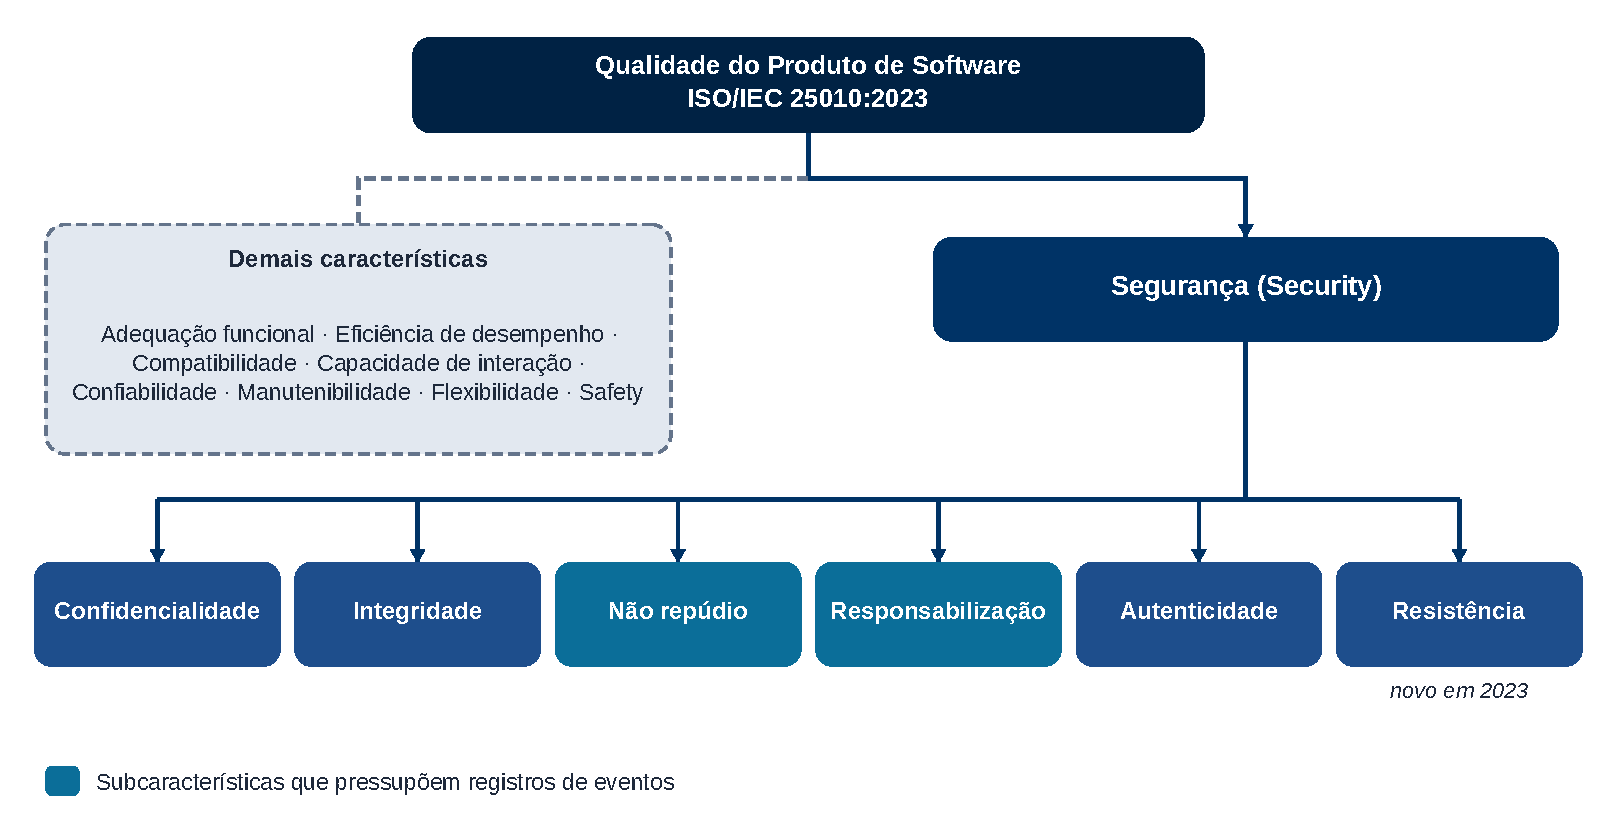
\includegraphics[width=0.92\textwidth]{figuras/iso25010_seguranca.eps}
    \fonte{Adaptado de \citeonline{iso25010_2023}.}
\end{figure}

As subcaracterísticas de não repúdio e de responsabilização pressupõem a existência de registros que identifiquem quem realizou determinada ação e quando. É nesse ponto que o atributo de qualidade se conecta aos registros de auditoria, tema da Seção~\ref{sec:ref_monitoramento_logs}.

No plano da gestão, a ISO/IEC 27001 estabelece os requisitos de um Sistema de Gestão da Segurança da Informação, orientado à preservação da confidencialidade, da integridade e da disponibilidade da informação \cite{iso27001_2022}. Entre os controles tecnológicos do Anexo A da edição de 2022 constam o registro de eventos (A.8.15), o monitoramento de atividades (A.8.16) e a sincronização de relógios (A.8.17) \cite{iso27001_2022}, que tratam, em termos gerais, da produção, proteção e análise de registros, da vigilância de comportamentos anômalos e da consistência temporal dos eventos.

A adoção de ciclos de integração e entrega contínuas alterou a forma de tratar a segurança. \citeonline{fitzgerald2017} descrevem a engenharia de software contínua como resposta à desconexão entre atividades como planejamento, desenvolvimento e implantação, e a prática de DevOps reconhece que a integração entre desenvolvimento e operação deve ser contínua. A abordagem DevSecOps estende essa integração à segurança. A revisão sistemática de \citeonline{rajapakse2022}, que analisou 54 estudos, identificou 21 desafios e 31 soluções na adoção de DevSecOps, com destaque para a necessidade de automatizar procedimentos manuais de segurança e para as práticas de avaliação contínua de segurança. Tais práticas incidem sobretudo sobre o \textit{pipeline} de entrega; a verificação do ambiente em operação, a partir dos registros que ele gera, é tratada nas seções seguintes.

\section{Arquiteturas Cloud-Native e Orquestração de Contêineres}
\label{sec:ref_cloud_native}

\subsection{Microsserviços e Contêineres}
\label{subsec:ref_microsservicos_conteineres}

\subsection{Orquestração de Contêineres com Kubernetes}
\label{subsec:ref_kubernetes}

\section{Monitoramento em Tempo de Execução e Gestão de Logs}
\label{sec:ref_monitoramento_logs}

\subsection{Gestão de Logs de Auditoria e Telemetria em \textit{Runtime}}
\label{subsec:ref_gestao_logs}

\subsection{Sistemas SIEM, HIDS e XDR}
\label{subsec:ref_siem_hids_xdr}

\subsection{Plataforma Wazuh}
\label{subsec:ref_wazuh}

\section{Conformidade Regulatória e Frameworks de Segurança}
\label{sec:ref_conformidade_normativa}

\subsection{CIS Critical Security Controls e o Controle 8}
\label{subsec:ref_cis_controls}

\subsection{PPSI 2.0, Computação em Nuvem e IN SGD/MGI nº 4/2026}
\label{subsec:ref_ppsi}

\subsection{Diretrizes Forenses de Registros: NC nº 21/IN01/DSIC/GSI-PR}
\label{subsec:ref_nc21}
